\chapter{功、能量与势能}\label{ch:b1:work-and-energy}

骑自行车的人在山顶停止蹬踏，到达山脚时的速率
只取决于高度落差，而与路面的形状无关。
蹦极者下落六十米，在某一瞬间停下，
恰在绳索的拉力吃掉了下落所积累的全部速率之处。
与氯原子结合的氢原子在一个\omterm{def:b1:work-and-energy:turning}{势阱}中振动，\omterm{def:b1:work-and-energy:turning}{势阱}的深度
即把分子拆开所需付出的能量。每种情形中都有一个
单一的量在不同形式之间交换——运动、高度、伸长、
化学键——将它们求和，其值保持不变。本章由牛顿第二定律出发，建立这套
核算：功与功率、\omterm{thm:b1:work-and-energy:ke}{动能}定理、
允许定义\omterm{def:b1:work-and-energy:conservative}{势能}的那些力的\omterm{def:b1:work-and-energy:conservative}{势能}，以及
\omterm{thm:b1:work-and-energy:em}{机械能守恒}，它使许多动力学问题化为
一行代数运算，并借助\omterm{def:b1:work-and-energy:turning}{势阱}的形状
说明哪些位置是稳定的。

\begin{omfigure}
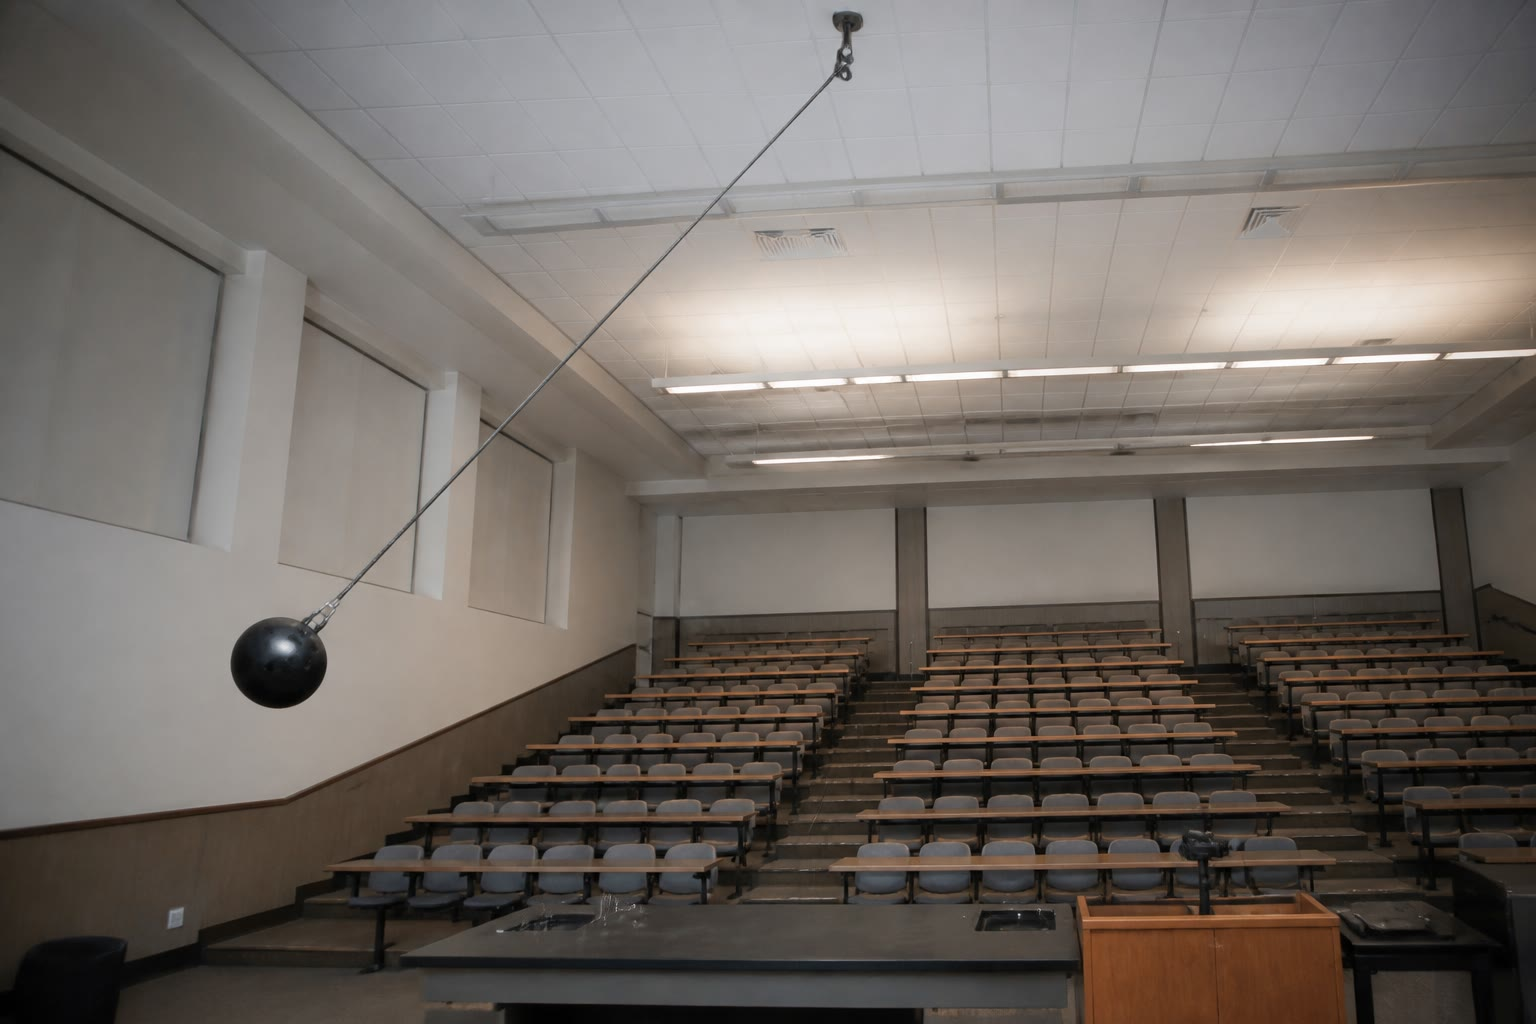
\includegraphics[width=0.58\linewidth]{images/book3/ai/b3-13-lecture-hall-pendulum.jpg}

{\small 讲台上的摆：保龄球从鼻尖处释放后回到鼻尖，不再越过此处——\omterm{thm:b1:work-and-energy:em}{机械能守恒}，且从未超过其初始值。}
\end{omfigure}

\section{功与功率}

\begin{definition}[力的功率与功]\label{def:b1:work-and-energy:work}
\index{功率}\index{功}
力的\emph{功率}是作用于质点上的力 $\vect F$ 与
质点速度 $\vect v$ 的点积，即
\[
\mathcal P = \vect F\cdot\vect v \qquad (\text{瓦特}),
\]
而力的\emph{功}在时刻 $t_1$ 至 $t_2$ 之间
（位置为 $A$ 与 $B$）是功率的累积，
\[
W_{A\to B} = \int_{t_1}^{t_2}\vect F\cdot\vect v\,\dd t
= \int_A^B \vect F\cdot\dd\vect\ell \qquad (\text{焦耳}),
\]
即\emph{元功} $\delta W = \vect F\cdot\dd\vect\ell$ 之和，
沿\omterm{def:b1:point-kinematics:frame}{轨迹}的元位移为 $\dd\vect\ell = \vect v\,\dd t$。
力沿运动方向推动时做正功，
（\emph{动力}），逆着运动方向时做负功（\emph{阻力}），垂直时
功为零。
\end{definition}

\begin{proposition}[常见的功]\label{prop:b1:work-and-energy:works}
\begin{itemize}
  \item 恒力：$W_{A\to B} = \vect F\cdot\vect{AB}$，与
        路径无关。重力：$W = mg(z_A - z_B)$，$z$ 竖直向上计数。
  \item 劲度系数为 $k$ 的弹簧，伸长量从 $x_A$ 变为 $x_B$：
        $W = \tfrac12 k(x_A^2 - x_B^2)$。
  \item 固定表面的\omterm{prop:b1:newton-dynamics:friction}{法向力}，以及绳子张力作用于
        沿垂直于该面方向运动的物体上：$W = 0$（力 $\perp$ 位移）。
  \item 动摩擦力与阻力：始终有 $W < 0$（力与
        相对运动方向相反），且与路径长度有关。
\end{itemize}
\end{proposition}

\begin{proof}
恒力 $\vect F$：$\int\vect F\cdot\dd\vect\ell = \vect F\cdot\int\dd\vect\ell
= \vect F\cdot\vect{AB}$；取 $\vect F = -mg\vect e_z$，$\vect F\cdot\vect{AB}
= -mg(z_B - z_A)$。弹簧：$\vect F\cdot\dd\vect\ell = -kx\,\dd x$，且
$\int_{x_A}^{x_B}-kx\,\dd x = \tfrac12 k(x_A^2 - x_B^2)$。摩擦力：$\vect T
= -\mu N\vect v/v$，故 $\vect T\cdot\vect v = -\mu Nv < 0$。
\end{proof}

\begin{omfigure}
\begin{tikzpicture}[font=\small, x=1cm, y=1cm]
  \draw[omDef, thick, domain=0:6, samples=60] plot (\x, {0.35*\x + 0.9*sin(deg(0.7*\x))});
  \fill (0,0) circle (1.4pt) node[below] {$A$};
  \fill (6,{2.1+0.9*sin(deg(4.2))}) circle (1.4pt) node[right] {$B$};
  % point at x=2.4: y = 0.84+0.9*sin(96.3deg)=0.84+0.894=1.734 ; slope 0.35+0.63cos(96.3)=0.35-0.069=0.28
  \coordinate (M) at (2.4,1.734);
  \fill[omThm] (M) circle (1.6pt); \node[above left] at (M) {$M$};
  \draw[-Stealth, omThm, very thick] (M) -- ++(1.1,0.31) node[right] {$\dd\vect\ell$};
  \draw[-Stealth, omProp, very thick] (M) -- ++(1.4,-0.9) node[below right] {$\vect F$};
  \draw ($(M)+(0.55,0.15)$) arc (15.6:-32.7:0.57); \node at ($(M)+(0.85,-0.12)$) {$\alpha$};
  \node[omExo, font=\footnotesize] at (3.6,3.4) {$\delta W = \vect F\cdot\dd\vect\ell = F\,\dd\ell\cos\alpha$};
\end{tikzpicture}

{\small 力沿其作用点一段小位移所做的元功：只有
$\vect F$ 沿运动方向的分量做功。
沿从 $A$ 到 $B$ 的路径求和，
即得 $W_{A\to B}$。}
\end{omfigure}

\section{动能定理}

\begin{theorem}[动能定理与功率定理]\label{thm:b1:work-and-energy:ke}
\index{动能}\index{动能定理}
在\omterm{thm:b1:newton-dynamics:laws}{惯性参考系}中，质点的\emph{\omterm{thm:b1:work-and-energy:ke}{动能}} $E_k = \tfrac12 mv^2$ 满足
以下关系：
\[
\frac{\dd E_k}{\dd t} = \sum\mathcal P_i = \Big(\sum\vect F_i\Big)\cdot\vect v,
\qquad
E_k(B) - E_k(A) = \sum_i W_{i,A\to B}:
\]
两位置之间\omterm{thm:b1:work-and-energy:ke}{动能}的变化量等于
沿途所有力所做功的总和。
\end{theorem}

\begin{proof}
将牛顿第二定律与 $\vect v$ 作点积：$m\vect a\cdot\vect v =
\tfrac{\dd}{\dd t}(\tfrac12 m\vect v\cdot\vect v) = \dd E_k/\dd t$，而
$(\sum\vect F_i)\cdot\vect v = \sum\mathcal P_i$。对时间积分即可。
\end{proof}

\begin{example}[制动距离]\label{ex:b1:work-and-energy:braking}
一辆质量为 \qty{1000}{kg} 的汽车以 \qty{100}{km/h} 的速率行驶（$E_k = \qty{386}{kJ}$），
在恒定的 \qty{7.0}{kN} 制动力作用下停止，其制动距离为 $d = E_k/F = \qty{55}{m}$：
距离随速率的\emph{平方}而增长。由于
最大制动力为 $\mu_smg$（见\cref{ch:b1:newton-dynamics}），
最短停车距离为 $v^2/2\mu_sg$，与汽车的质量无关——
在湿滑路面上 $\mu_s$ 减半，停车距离则加倍。
\end{example}

\section{保守力与势能}

\begin{definition}[保守力；势能]\label{def:b1:work-and-energy:conservative}
\index{保守力}\index{势能}
若一个力在两点之间所做的功不
依赖于所经路径，则称该力为\emph{保守力}。等价地，存在一个位置的函数，
即\emph{势能}$E_p$，使得
\[
W_{A\to B} = E_p(A) - E_p(B) = -\Delta E_p ,
\qquad \delta W = -\dd E_p ,
\]
$E_p$ 只确定到一个加性常数（即零点的选取）。
\end{definition}

\begin{proposition}[由势能求力]\label{prop:b1:work-and-energy:gradient}
\index{梯度}
\omterm{def:b1:work-and-energy:conservative}{保守力}由其\omterm{def:b1:work-and-energy:conservative}{势能}导出：
\[
\vect F = -\overrightarrow{\operatorname{grad}}\,E_p
= -\frac{\partial E_p}{\partial x}\,\vect e_x
- \frac{\partial E_p}{\partial y}\,\vect e_y
- \frac{\partial E_p}{\partial z}\,\vect e_z ,
\]
在一维情形下 $F_x = -\dd E_p/\dd x$：力指向
\omterm{def:b1:work-and-energy:conservative}{势能}减小的方向，即 $E_p$ 图像上的“下坡”方向。
\end{proposition}

\begin{proof}
$\delta W = F_x\dd x + F_y\dd y + F_z\dd z = -\dd E_p = -(\partial_xE_p\,\dd x
+ \partial_yE_p\,\dd y + \partial_zE_p\,\dd z)$ 对任意位移成立：
由位移的任意性比较各项系数（用到数学课程中关于
多元函数的微分）。
\end{proof}

\begin{proposition}[常见势能]\label{prop:b1:work-and-energy:eps}
\index{势能!引力}\index{势能!弹性}
\begin{itemize}
  \item 重力：$E_p = mgz + \text{常数}$（$z$ 轴竖直向上）。
  \item 弹簧：$E_p = \tfrac12 k(\ell - \ell_0)^2 + \text{常数}$。
  \item 质量为 $M$ 的物体产生的牛顿万有引力：$E_p = -GMm/r + \text{常数}$，
        通常选取常数，使 $E_p \to 0$ 于无穷远处。
  \item 电荷 $q$ 在电势 $V$ 中所受的静电力：
        $E_p = qV$（见\cref{ch:b1:potential-capacitors}）。
\end{itemize}
动摩擦力与流体阻力都\emph{不是}\omterm{def:b1:work-and-energy:conservative}{保守力}（它们所做的功
与路径有关，且总是负的）。
\end{proposition}

\begin{proof}
各式均可由\cref{prop:b1:work-and-energy:works}中各力的功直接读出：
$W = -\Delta E_p$。对于万有引力，$\vect F = -GMm/r^2\,\vect e_r$，且
$\delta W = -GMm\,\dd r/r^2 = -\dd(-GMm/r)$.
\end{proof}

\section{机械能}

\begin{theorem}[机械能]\label{thm:b1:work-and-energy:em}
\index{机械能}\index{机械能守恒}
记 $E_m = E_k + E_p$ 为\emph{\omterm{thm:b1:work-and-energy:em}{机械能}}，其中 $E_p$ 为
各\omterm{def:b1:work-and-energy:conservative}{保守力}\omterm{def:b1:work-and-energy:conservative}{势能}之和。于是
\[
\Delta E_m = W_{\text{非保守}} ,
\]
非\omterm{def:b1:work-and-energy:conservative}{保守力}所做的总功。若这些力不做功
（无摩擦，或约束力与运动垂直），则 $E_m$
是\emph{守恒}的，即运动为\emph{保守}运动。
\end{theorem}

\begin{proof}
$\Delta E_k = W_{\text{c}} + W_{\text{非保守}} = -\Delta E_p + W_{\text{非保守}}$.
\end{proof}

\begin{method}[用能量求解]\label{met:b1:work-and-energy:method}
当问题要求\emph{某位置处的速率}（而非时间，也非
力）时，应先尝试能量方法：
\begin{enumerate}
  \item 列出各力，判断哪些力做功、哪些力是\omterm{def:b1:work-and-energy:conservative}{保守力}；
  \item 写出两位置处的 $E_m$，并明确 $E_p$ 的零点；
        \item 令两者相等（若有摩擦力作用，则计入 $W_{\text{非保守}}$），并
        解出未知的速率或位置。
\end{enumerate}
能量方法不能给出时间或约束力；求这些量时，
应回到牛顿定律，常常利用刚由能量方法求得的速率。
\end{method}

\begin{example}[圆环轨道的速率规律]\label{ex:b1:work-and-energy:loop}
在\cref{pb:b1:point-kinematics:1}中的无摩擦圆环上，轨道的
\omterm{prop:b1:newton-dynamics:friction}{法向力}与运动方向垂直、不做功：$E_m$ 守恒。
取 $z = R(1 - \cos\theta)$ 为相对最低点的高度，$\tfrac12 mv^2 + mgR(1 -
\cos\theta) = \tfrac12 mv_0^2$，即速率规律 $v^2 = v_0^2 - 2gR(1 -
\cos\theta)$ 前文已用过，现在一行即可导出。入口处的最小速率
为 $\sqrt{5gR}$，它由最高点条件
$v^2 \geq gR$（见\cref{ex:b1:newton-dynamics:circles}）导出。
\end{example}

\begin{example}[摩擦损失的能量]\label{ex:b1:work-and-energy:friction}
一物块沿倾角为 $\alpha$、高为 $h$ 的斜面下滑，
动\omterm{prop:b1:newton-dynamics:friction}{摩擦因数}为 $\mu_d$：$W_{\text{非保守}} = -\mu_dmg\cos\alpha \times
h/\sin\alpha = -\mu_dmgh\cot\alpha$，故 $\tfrac12 mv^2 = mgh(1 - \mu_d\cot\alpha)$。
取 $h = \qty{2.0}{m}$，$\alpha = 30^\circ$，$\mu_d = 0.20$，则 $v =
\qty{5.1}{m/s}$，而非 $\qty{6.3}{m/s}$；\omterm{def:b1:work-and-energy:conservative}{势能}的三分之一
转化为热量。
\end{example}

\section{平衡、稳定性与相图}

\begin{proposition}[一维情形下的平衡与稳定性]\label{prop:b1:work-and-energy:stability}
\index{平衡!稳定、不稳定}\index{小振动}
一质点沿一条坐标轴运动，受
\omterm{def:b1:work-and-energy:conservative}{势能}为 $E_p(x)$ 的\omterm{def:b1:work-and-energy:conservative}{保守力}作用：
\begin{itemize}
  \item 质点处于\emph{平衡}，位置为 $x_0$，当且仅当 $F(x_0) = -E_p'(x_0) = 0$：
        即 $E_p$ 的极值点；
  \item 平衡为\emph{稳定}的，若 $E_p$ 在该点取局部极小
        值（$E_p''(x_0) > 0$）：小位移产生
        回复力；在极大值处则为\emph{不稳定}的。
  \item 在稳定平衡点附近，微小运动是简谐的，且满足
        \[
        \omega_0^2 = \frac{E_p''(x_0)}{m} .
        \]
\end{itemize}
\end{proposition}

\begin{proof}
由泰勒公式（数学课程）：$E_p(x) \approx E_p(x_0) +
\tfrac12 E_p''(x_0)(x - x_0)^2$，于是 $F \approx -E_p''(x_0)(x - x_0)$，
即 $m\ddot x = -E_p''(x_0)(x - x_0)$——相当于劲度系数为 $E_p''(x_0)$ 的弹簧。
若 $E_p'' < 0$，则“劲度系数”为负：偏离呈指数增长。
\end{proof}

\begin{omfigure}
\begin{tikzpicture}
\begin{axis}[omaxis, axis x line=bottom, axis y line=left, width=10.5cm, height=5.8cm, xlabel={$x$}, ylabel={$E_p$},
    xlabel style={at={(axis description cs:0.5,-0.06)}, anchor=north},
    xmin=-2.3, xmax=2.5, ymin=-1.5, ymax=1.6, xtick={-1,1}, xticklabels={$-a$,$a$}, ytick=\empty]
  \addplot[omDef, thick, domain=-2.15:2.15, samples=200] {x^4 - 2*x^2 + 0.3*x};
  \addplot[omThm, dashed, domain=-2.3:2.5, samples=2] {-0.45};
  \addplot[omExo, dashed, domain=-2.3:2.5, samples=2] {0.9};
  \node[omThm, font=\footnotesize, anchor=east] at (axis cs:2.45,-0.3) {$E_1$};
  \node[omExo, font=\footnotesize, anchor=east] at (axis cs:2.45,1.05) {$E_2$};
  \node[font=\footnotesize, below] at (axis cs:-1.08,-0.7) {稳定};
  \node[font=\footnotesize, above] at (axis cs:0.08,0.08) {不稳定};
  \node[font=\footnotesize, below] at (axis cs:0.97,-1.1) {稳定};
  \draw[Stealth-Stealth, omThm] (axis cs:-1.56,-0.45) -- (axis cs:-0.47,-0.45);
  \draw[Stealth-Stealth, omThm] (axis cs:0.42,-0.45) -- (axis cs:1.48,-0.45);
\end{axis}
\end{tikzpicture}

{\small 一维\omterm{def:b1:work-and-energy:conservative}{势能}图景：极小值为稳定平衡点，
极大值为不稳定平衡点。能量为 $E_1$ 的质点位于\omterm{def:b1:work-and-energy:turning}{势垒}之下，
被困在一个\omterm{def:b1:work-and-energy:turning}{势阱}中，位于两个\emph{\omterm{def:b1:work-and-energy:turning}{转折
点}}之间（其中 $E_p = E_1$，即箭头所示处），并做振动；能量 $E_2$ 高于
\omterm{def:b1:work-and-energy:turning}{势垒}，质点可自由地从一个\omterm{def:b1:work-and-energy:turning}{势阱}越到另一个。}
\end{omfigure}

\begin{definition}[转折点；束缚运动与自由运动]\label{def:b1:work-and-energy:turning}
\index{转折点}\index{束缚运动}\index{势阱}\index{势垒}
对能量为 $E_m$ 的保守一维运动，质点
只能位于 $E_p(x) \leq E_m$ 的区域（因为 $E_k \geq 0$）；满足
$E_p = E_m$ 的点称为\emph{转折点}，在该处速度为零并反向。
若质点被困于两个转折点之间的\emph{势阱}中，则运动为
\emph{束缚}的且是周期的；若能到达无穷远，则为\emph{自由}的；
能量高于 $E_m$ 的\emph{势垒}
无法越过。
\end{definition}

\begin{definition}[相图]\label{def:b1:work-and-energy:phase}
\index{相图}
一维运动的\emph{相图}是点 $(x, \dot x)$
在\emph{相平面}中描出的一族曲线。对保守系统，每条曲线都是等值线
$\tfrac12 m\dot x^2 +
E_p(x) = E_m$：围绕稳定平衡点的为闭曲线（振动），
自由运动对应开曲线，而经过不稳定平衡点的则是将两者分开的
\emph{分界线}。曲线按顺时针方向运行
（$\dot x > 0$ 表示 $x$ 增大），且互不相交。
\end{definition}

\begin{omfigure}
\begin{tikzpicture}
\begin{axis}[omaxis, width=11cm, height=6.2cm, xlabel={$\theta$}, ylabel={$\dot\theta/\omega_0$},
    xmin=-7.2, xmax=7.2, ymin=-2.6, ymax=2.6, xtick={-6.283,-3.1416,0,3.1416,6.283},
    xticklabels={$-2\pi$,$-\pi$,$0$,$\pi$,$2\pi$}, ytick={-2,2}]
  % closed curves: thetadot^2 = 2(e - (1 - cos theta)) with e<2 ; thetadot = ±sqrt(2(e-1+cos))
  \foreach \e/\tm in {0.3/0.795, 1.0/1.5708, 1.7/2.346} {
    \foreach \sh in {0, 6.2832, -6.2832} {
      \addplot[omDef, thick, domain=-\tm:\tm, samples=200] ({x+\sh},{sqrt(max(0,2*(\e-1+cos(deg(x)))))});
      \addplot[omDef, thick, domain=-\tm:\tm, samples=200] ({x+\sh},{-sqrt(max(0,2*(\e-1+cos(deg(x)))))});
    }
  }
  % separatrix e=2
  \addplot[omThm, thick, domain=-7.2:7.2, samples=400] {sqrt(2*(1+cos(deg(x))))};
  \addplot[omThm, thick, domain=-7.2:7.2, samples=400] {-sqrt(2*(1+cos(deg(x))))};
  % rotations e=2.5, 3.2
  \foreach \e in {2.6,3.4} {
    \addplot[omProp, thick, domain=-7.2:7.2, samples=300] {sqrt(2*(\e-1+cos(deg(x))))};
    \addplot[omProp, thick, domain=-7.2:7.2, samples=300] {-sqrt(2*(\e-1+cos(deg(x))))};
  }
  \fill (axis cs:0,0) circle (1.5pt); \fill (axis cs:3.1416,0) circle (1.5pt); \fill (axis cs:-3.1416,0) circle (1.5pt);
\end{axis}
\end{tikzpicture}

{\small \omterm{ex:b1:newton-dynamics:pendulum}{单摆}的\omterm{def:b1:work-and-energy:phase}{相图}，$\tfrac12\dot\theta^2 +
\omega_0^2(1 - \cos\theta) = \text{常量}$。闭曲线（蓝色）：绕稳定平衡点
$\theta = 0$ 摆动；开曲线（橙色）：完整转动；
两者之间的分界线（红色）经过不稳定平衡点
$\theta = \pm\pi$，对应恰好能到达最高点的运动。}
\end{omfigure}

\begin{example}[单摆的势能图景]\label{ex:b1:work-and-energy:pendulum}
$E_p = -mg\ell\cos\theta$：在 $\theta = 0$ 处取极小值，$E_p'' = mg\ell$，于是
$\omega_0^2 = g\ell/(m\ell^2) = g/\ell$——这是由\omterm{def:b1:work-and-energy:turning}{势阱}曲率读出的
\cref{ex:b1:newton-dynamics:pendulum} 中\omterm{prop:b1:work-and-energy:stability}{小振动}的结果；
在 $\theta = \pi$ 处取极大值，即倒立摆，为不稳定的。能量
$E_m < mg\ell$ 时在 $\pm\theta_{\max}$ 之间振动；$E_m > mg\ell$ 时，
越过最高点并转动；$E_m = mg\ell$ 时为分界线，
质点无限缓慢地趋近最高点。
\end{example}

\section{练习}

\begin{exercise}[$\star$]\label{exo:b1:work-and-energy:1}
一个质量为 \qty{20}{kg} 的箱子在
\qty{5.0}{s} 内匀速被提升 \qty{3.0}{m}。求提升力、重力所做的功，以及所提供的功率。
同一箱子沿地面被推动 \qty{3.0}{m}，地面的
动\omterm{prop:b1:newton-dynamics:friction}{摩擦因数} $\mu_d = 0.30$：求摩擦力所做的功。
\end{exercise}

\begin{exercise}[$\star$]\label{exo:b1:work-and-energy:2}
求质量为 \qty{1000}{kg} 的汽车以 \qty{100}{km/h} 行驶时的\omterm{thm:b1:work-and-energy:ke}{动能}；
在恒定的 \qty{7.0}{kN} 制动力下的停车距离；
若速率加倍，则停车距离将如何变化？
\end{exercise}

\begin{exercise}[$\star$]\label{exo:b1:work-and-energy:3}
一个劲度系数为 \qty{500}{N/m} 的弹簧被压缩 \qty{10}{cm}，
然后释放，推动位于光滑水平轨道上的一个 \qty{50}{g} 的小球。
求弹簧储存的能量以及小球的速率。
\end{exercise}

\begin{exercise}[$\star$]\label{exo:b1:work-and-energy:4}
一根长为 \qty{1.0}{m} 的\omterm{ex:b1:newton-dynamics:pendulum}{单摆}，从偏角为 $60^\circ$ 处由静止释放：
利用能量求最低点的速率；再利用牛顿第二定律求该处的张力
（以 $mg$ 为单位）。
\end{exercise}

\begin{exercise}[$\star\star$]\label{exo:b1:work-and-energy:5}
一个物块从静止开始沿高为 \qty{2.0}{m}、倾角为 $30^\circ$ 的斜面下滑，
设 $\mu_d = 0.20$。利用\omterm{thm:b1:work-and-energy:ke}{动能}定理求其到达底部时的速率；求
初始\omterm{def:b1:work-and-energy:conservative}{势能}中因摩擦而损失的比例。
\end{exercise}

\begin{exercise}[$\star\star$]\label{exo:b1:work-and-energy:6}
利用 $E_p = -GMm/r$，证明从地球表面逃离地球引力所需的速率
为 $v_e = \sqrt{2GM/R}$，并计算其数值
（$M = \qty{5.97e24}{kg}$，$R = \qty{6.37e6}{m}$）。若一天体的密度相同而半径为地球的两倍，
其逃逸速率是多少？
\end{exercise}

\begin{exercise}[$\star\star$]\label{exo:b1:work-and-energy:7}
蹦极：一名质量为 \qty{70}{kg} 的跳跃者，系着自然长度为 \qty{20}{m} 的绳索，
绳索劲度系数为 \qty{50}{N/m}，从静止开始跳下。求绳索的最大伸长量、总下落距离，
以及最大张力（以重力为单位）。
速率在何处最大？
\end{exercise}

\begin{exercise}[$\star\star$]\label{exo:b1:work-and-energy:8}
一名骑车人（连车共 \qty{80}{kg}）以 \qty{5.0}{m/s} 的速率爬上坡度为 $5\%$ 的斜坡，
并受阻力 $\tfrac12\rho C_xSv^2$ 作用，其中 $C_xS = \qty{0.50}{m^2}$。
求克服重力做功的功率、克服阻力做功的功率以及总功率。
\end{exercise}

\begin{exercise}[$\star\star$]\label{exo:b1:work-and-energy:9}
质量为 $m$ 的质点，其\omterm{def:b1:work-and-energy:conservative}{势能}为 $E_p(x) = E_0[(x/a)^4 - 2(x/a)^2]$。
求平衡位置及其稳定性、\omterm{def:b1:work-and-energy:turning}{势阱}的深度，
以及绕稳定平衡位置做\omterm{prop:b1:work-and-energy:stability}{小振动}的\omterm{def:b1:wave-propagation:signal}{角频率}。
\end{exercise}

\begin{exercise}[$\star\star\star$]\label{exo:b1:work-and-energy:10}
对于谐振子 $E_p = \tfrac12 kx^2$，证明其相曲线为椭圆，
给出能量为 $E$ 时的半轴长，
并说明为何所有相曲线都以相同的周期绕行。
\end{exercise}

\begin{exercise}[$\star\star\star$]\label{exo:b1:work-and-energy:11}
一个小物体从光滑半球顶端由静止开始下滑，半球半径为 $R$。
利用能量和牛顿第二定律，求物体离开球面处与竖直方向的夹角、
该处的高度，
以及该处的速率。
\end{exercise}

\begin{exercise}[$\star\star\star$]\label{exo:b1:work-and-energy:12}
一辆以 \qty{90}{km/h} 行驶的汽车，车轮抱死后
滑行 \qty{80}{m} 停止。利用能量求 $\mu_d$。能量去了哪里？
为什么装有防抱死系统（车轮保持滚动）的汽车停车距离更短？
\end{exercise}

\section{问题：化学键的能谷}

\begin{problem}[{周末问题——两个原子，一条曲线：把化学键的势能读作一片地形——
它的谷底、谷壁，
谷底附近的微小振动，以及爬出谷底所需的能量}]
\label{pb:b1:work-and-energy:1}
双原子分子中两个原子的相互作用，
可用如下\omterm{def:b1:work-and-energy:conservative}{势能}描述：
\[
E_p(r) = \epsilon\left[\left(\frac{\sigma}{r}\right)^{12} - 2\left(\frac{\sigma}{r}\right)^{6}\right],
\]
$r$ 为两原子核之间的距离。对于氯化氢，取
$\epsilon = \qty{4.4}{eV}$，$\sigma = \qty{0.127}{nm}$，并令较轻的
氢原子（$m = \qty{1.67e-27}{kg}$）运动，而较重的氯原子保持不动。
$\qty{1}{eV} = \qty{1.60e-19}{J}$；$k_B = \qty{1.38e-23}{J/K}$；
$N_A = \num{6.02e23}$。

\medskip
\noindent\textbf{第一部分——能谷。}
\begin{enumerate}
  \item 求 $E_p$ 在 $r \to 0$ 与 $r \to \infty$ 时的极限，并
        画出曲线的草图。
  \item 证明 $E_p$ 仅有一个极小值，位于 $r = \sigma$ 处，其值为
        $-\epsilon$。
  \item 令 $u = (\sigma/r)^6$，证明 $E_p = \epsilon(u^2 - 2u)$，它是关于 $u$ 的
        抛物线。由此求出极小值。
  \item 用 $F(r)$ 表示力（排斥时取正），并给出其
        在 $\sigma$ 两侧的符号。
  \item 求 $E_p$ 与 $F$ 在 $r = 1.2\sigma$ 处的值（分别以 eV 和 nN 为单位）。
  \item 该分子的解离能为多少？请分别以 eV 和
        \unit{kJ/mol} 表示。（HCl 键能的实测值为 \qty{431}{kJ/mol}。）
  \item 检验 $r = \sigma$ 处的稳定性判据：计算
        $E_p''(\sigma)$。
\end{enumerate}

\medskip
\noindent\textbf{第二部分——\omterm{prop:b1:work-and-energy:stability}{小振动}。}
\begin{enumerate}[resume]
  \item 写出 $E_p$ 在 $\sigma$ 处的二阶泰勒展开式，
        并确定等效劲度系数 $k$。
  \item 求 $k$（以 \unit{N/m} 为单位）。
  \item 由此求出振动的\omterm{def:b1:wave-propagation:signal}{角频率}、频率和波长，
        以及以 \unit{cm^{-1}} 为单位的\omterm{prop:b1:wave-propagation:sinusoidal}{波数} $1/\lambda$。
  \item HCl 的实测振动\omterm{prop:b1:wave-propagation:sinusoidal}{波数}为 \qty{2990}{cm^{-1}}。请评论
        两者的符合情况，以及该模型正确之处。
  \item 在 \qty{300}{K} 时，平均振\omterm{thm:b1:work-and-energy:ke}{动能}量的\omterm{def:b1:units-dimensions:oom}{数量级}为 $k_BT$。
        估计振动\omterm{def:b1:wave-propagation:signal}{振幅}，并与 $\sigma$ 作比较。
  \item 由此求出该振动中氢原子的最大
        速率。
\end{enumerate}

\medskip
\noindent\textbf{第三部分——大\omterm{def:b1:wave-propagation:signal}{振幅}振动及其出路。}
\begin{enumerate}[resume]
  \item 描述\omterm{def:b1:work-and-energy:phase}{相图}：哪些能量对应闭合曲线，
        哪些对应开曲线，又是什么将二者分开？
  \item 对 $E_m = -\epsilon/2$，求两个\omterm{def:b1:work-and-energy:turning}{转折点}（以
        $\sigma$ 为单位）。
  \item 证明两\omterm{def:b1:work-and-energy:turning}{转折点}的中点位于 $\sigma$ 之外，并说明为何
        加热（提高振\omterm{thm:b1:work-and-energy:ke}{动能}量）会使平均键
        长增大，这正是热膨胀的根源。
  \item 大\omterm{def:b1:wave-propagation:signal}{振幅}振动的周期比
        $2\pi/\omega_0$ 更长还是更短？请从势壁的形状加以论证。
  \item 由 $E_m = -\epsilon/2$ 出发，需要提供多少能量
        才能使分子解离？若以氢原子在 $r = \sigma$ 处的\omterm{thm:b1:work-and-energy:ke}{动能}给出，
        则对应的速率是多少？
  \item 两个原子从远处相向靠近，总能量为正，
        仅靠自身不能形成束缚态分子。为什么？还需要什么？
\end{enumerate}

\medskip
\noindent\textbf{第四部分——功、力与温度。}
\begin{enumerate}[resume]
  \item 计算 $r$ 从 $2\sigma$ 变到
        $\sigma$ 时键力所做的功。该处的键力是动力还是阻力？
  \item 计算外部作用者须做的功，使键
        以趋近于零的速率从 $\sigma$ 拉伸到 $1.5\sigma$。
  \item 计算 $F$ 在 $r = 0.9\sigma$ 处的值，并与
        $r = 1.2\sigma$ 处作比较：这种不对称性说明了压缩与拉伸有何区别？
  \item $k_BT$ 等于 $\epsilon$ 时对应的温度为多少？为什么
        实际中分子在低得多的温度下就会解离？
  \item 一个更好的模型（莫尔斯势）改变了势壁的形状，但保持
        键长处的极小值。上述结果中哪些在方法上依然适用，
        哪些数值会发生变化？
  \item 总结能量方法的三种用途：求平衡位置，
        求振动频率，以及求
        解离所需的条件。
\end{enumerate}
\end{problem}
